\documentclass{vgtc}                          % final (conference style)
%\documentclass[review]{vgtc}                 % review
%\documentclass[widereview]{vgtc}             % wide-spaced review
%\documentclass[preprint]{vgtc}               % preprint
%\documentclass[electronic]{vgtc}             % electronic version

%% Uncomment one of the lines above depending on where your paper is
%% in the conference process. ``review'' and ``widereview'' are for review
%% submission, ``preprint'' is for pre-publication, and the final version
%% doesn't use a specific qualifier. Further, ``electronic'' includes
%% hyperreferences for more convenient online viewing.

%% Please use one of the ``review'' options in combination with the
%% assigned online id (see below) ONLY if your paper uses a double blind
%% review process. Some conferences, like IEEE Vis and InfoVis, have NOT
%% in the past.

%% Figures should be in CMYK or Grey scale format, otherwise, colour 
%% shifting may occur during the printing process.

%% These few lines make a distinction between latex and pdflatex calls and they
%% bring in essential packages for graphics and font handling.
%% Note that due to the \DeclareGraphicsExtensions{} call it is no longer necessary
%% to provide the the path and extension of a graphics file:
%% \includegraphics{diamondrule} is completely sufficient.
%%
\ifpdf%                                % if we use pdflatex
  \pdfoutput=1\relax                   % create PDFs from pdfLaTeX
  \pdfcompresslevel=9                  % PDF Compression
  \pdfoptionpdfminorversion=7          % create PDF 1.7
  \ExecuteOptions{pdftex}
  \usepackage{graphicx}                % allow us to embed graphics files
  \DeclareGraphicsExtensions{.pdf,.png,.jpg,.jpeg} % for pdflatex we expect .pdf, .png, or .jpg files
\else%                                 % else we use pure latex
  \ExecuteOptions{dvips}
  \usepackage{graphicx}                % allow us to embed graphics files
  \DeclareGraphicsExtensions{.eps}     % for pure latex we expect eps files
\fi%

%% it is recomended to use ``\autoref{sec:bla}'' instead of ``Fig.~\ref{sec:bla}''
\graphicspath{{figures/}{pictures/}{images/}{./}} % where to search for the images

\usepackage{microtype}                 % use micro-typography (slightly more compact, better to read)
\PassOptionsToPackage{warn}{textcomp}  % to address font issues with \textrightarrow
\usepackage{textcomp}                  % use better special symbols
\usepackage{mathptmx}                  % use matching math font
\usepackage{times}                     % we use Times as the main font
\renewcommand*\ttdefault{txtt}         % a nicer typewriter font
\usepackage{cite}
\usepackage{graphicx}   
           % needed to automatically sort the references
%% We encourage the use of mathptmx for consistent usage of times font
%% throughout the proceedings. However, if you encounter conflicts
%% with other math-related packages, you may want to disable it.


%% If you are submitting a paper to a conference for review with a double
%% blind reviewing process, please replace the value ``0'' below with your
%% OnlineID. Otherwise, you may safely leave it at ``0''.
\onlineid{0}

%% declare the category of your paper, only shown in review mode
\vgtccategory{Research}

%% allow for this line if you want the electronic option to work properly


%% In preprint mode you may define your own headline.
%\preprinttext{To appear in an IEEE VGTC sponsored conference.}

%% Paper title.

\title{Group 5 Project Proposal}


%% Author and Affiliation (multiple authors with multiple affiliations)

\author{Chethram Ramoutar\\ %
    \parbox{1.4in}{\scriptsize  \centering\emph{Hunter College}}\\
    \scriptsize{chethram.ramoutar79@myhunter.cuny.edu}
\and Melanie Vasquez\\ %
    \parbox{1.4in}{\scriptsize \centering\emph{Hunter College}}\\
    \scriptsize{melanie.vasquez61@myhunter.cuny.edu}
\and Omar Hegazy\\ %
    \parbox{1.4in}{\scriptsize  \centering\emph{Hunter College}}\\
    \scriptsize{omar.hegazy00@myhunter.cuny.edu}\\
\and Mark Blinder\\ %
    \parbox{1.4in}{\scriptsize  \centering\emph{Hunter College}}\\
    \scriptsize{mark.blinder54@myhunter.cuny.edu}}
%% A teaser figure can be included as follows, but is not recommended since
%% the space is now taken up by a full width abstract.
%\teaser{
%  \includegraphics[width=1.5in]{sample.eps}
%  \caption{Lookit! Lookit!}
%}

%% Abstract section.
\abstract{
With the growth of VR devices being more accessible to the masses, it is understood that environment,
interactivity, and the ability to immerse oneself in a virtual world is a key factor in the success of any
VR experience. However, achieving this experience is often difficult for many games due to lack of attention to interactivity
and immersion. In order to combat this, our group seeks to develop a VR game that will use hand input to immerse a user
in a quest-like game. To achieve immersion and interactivity we will use different tools and methodologies to help the player feel
like they are apart of the experience.%
} % end of abstract

%% ACM Computing Classification System (CCS). 
%% See <http://www.acm.org/about/class> for details.
%% We recommend the 2012 system <http://www.acm.org/about/class/class/2012>
%% For the 2012 system use the ``\CCScatTwelve'' which command takes four arguments.
%% The 1998 system <http://www.acm.org/about/class/class/2012> is still possible
%% For the 1998 system use the ``\CCScat'' which command takes four arguments.
%% In both cases the last two arguments (1998) or last three (2012) can be empty.


%% Copyright space is enabled by default as required by guidelines.
%% It is disabled by the 'review' option or via the following command:
% \nocopyrightspace

%%%%%%%%%%%%%%%%%%%%%%%%%%%%%%%%%%%%%%%%%%%%%%%%%%%%%%%%%%%%%%%%
%%%%%%%%%%%%%%%%%%%%%% START OF THE PAPER %%%%%%%%%%%%%%%%%%%%%%
%%%%%%%%%%%%%%%%%%%%%%%%%%%%%%%%%%%%%%%%%%%%%%%%%%%%%%%%%%%%%%%%%

\begin{document}
\maketitle
%% The ``\maketitle'' command must be the first command after the
%% ``\begin{document}'' command. It prepares and prints the title block.

%% the only exception to this rule is the \firstsection command
\firstsection{Introduction}


%% \section{Introduction} %for journal use above \firstsection{..} instead
The game centers around a lone space traveler who is on a quest to gather different supplies for a stranger on their ship. As they travel through
different dimensions, the user will experience different terrains, forms of life, and interesting settings. This game will be broken up into four key
areas of travel being: A desert, a forest, a village, and a farm. Each area's focus will allow us to give the user multiple cohesive experiences without
the risk of throwing them off from the main story. This will also allow the developers to test different aspects of each environment to present the idea that
a user truly traveled a different dimension.

Along with the environment, we seek to have non-playable character or NPC interaction that will make each space more lively and natural to the user. The NPC will be used as our stranger on the ship who will tell us what items
we must use and how many we should collect. This NPC will be animated but we will look into having other NPCs within different sections of the environmet. However, the main
functionality and interactivity will be with the quests assigned in each area. The user will be able to collect items that relate to their respective quest and explore a majority
of their environment to seek these out. Although it is simple, it can allow the user to immerse themselves without streinuous tasks breaking their immersion. The quests will be entirely focused on
hand input allowing a user to pick up, examine, and collect objects with ease. The user will also be able to look around and navigate the each environment as naturally as possible.

\section{Related Work}
Games that inspired the creation of this project are "The Witness"\cite{rad_2016} and "The Forest"\cite{hafer_2018,horti_2018}. "The Witness" uses environment and puzzle interaction in a seemless way and has been praised for having "masterful design"\cite{rad_2016}.
Integration of this in VR has translated well since the game was first published. By looking at how "The Witness" makes the environment the main aspect, it is something we want to take away from. Despite most if not all of the environment being in low poly 3D graphics, the
use of ray tracing, saturated colors, and a lack of clutter makes the environment feel alive and natural. The game also uses a first person perspective which is something we want to take away from. The first person perspective allows for a more
personal and intimate experience with the puzzles that is not often seen in VR games. There is more naturality with this view then with third person perspective.

"The Forest" also uses the previous aspects but in a more realistic and intense setting. The main aspects to take away from is the environmental interaction. Although "The Witness" achieves the appropriate aesthetic while integrating puzzles, "The Forest"
is more realistic with its gameplay. As stated by Samuel Horti: "Your inventory is just all your items laid on a mat in front of you, and the crafting menu is a book you pull out of your backpack. But being surrounded by the world on all sides in VR makes it more believable"\cite{horti_2018}.
Noting this and the ability to interact with tools such as axes, sticks, and even a bow and arrow brings a lot into the immersion of the game. Movement becomes key in the gameplay which is translated through the well thought out head and hand tracking
that makes every swing or flick feel meaningful in the environment the player is in. Since it is also a survival game, first person perspective brings out the sense of urgency
with every interaction. The game also contains well thought out NPC interactions that are extremely heart racing in a VR environment. By seeing how "The Forest" uses interactivity in its gameplay we want to try and achieve that within our game through our collection
quests. However, we want to keep the calmness and aesthic found in "The Witness" to make the game more enjoyable.

\subsection*{Interactivity Applications}

\section{Methodology}
In order to complete the project, it will be done on Unity 2021.3.7f1. All testing will occur with the Oculus Quest 1 and the Oculus Quest 2. Each scene will utilize assets from the Unity Asset Store and any other
source containing appropriate assets. The scenes will be connected through a main hub area which will contain teleportation pads to each area. The user will be able to teleport by standing on a pad and triggering
a script or pressing a button. These portals will also be placed in each area
in order to travel back to allow the user to have a choice on where to go.This will allow us to merge the scenes in a manner that fits with the story but also reduces any streinuous load times that may
occur.

Outside of the hub being worked on, each group member will handle a scene and quest that corresponds with it. The scenes will be split as so:
\begin{itemize}
  \item Desert: Melanie Vasquez
  \item Forest: Mark Blinder
  \item Village: Omar Hegazy
  \item Farm: Chethram Ramoutar
\end{itemize}

Interactivity will be integrated into each scene through the use of the XR rig and XR Interaction Toolkit. This rig will allow for VR testing due to the headset detection built into it and controller support allowing us to add eye and hand detection.
Along with that, the use of the XR Device Simulator will help with non-vr testing to take place throughout the debugging process since we can tweak any features without the full need of a VR headser. The XR Interaction Toolkit will allow for the user to
interact with objects in the scene by using their hands or eyes and will help us with the main portion of the interactivity. Since we are using hands as the main input device, having this allows us to test and enhance interaction experience with either haptic feedback
or visual feedback. This can help build upon each scene once we get into NPC interactions as well and ways the user can have the illusion of communication within each area.

Outside of the interactivity, for immersion we will use assets and different light and rendering techniques to allow a user to be in a space that is not dull. Animations will also be used because it can give the illusion of movement which can add life to each scene.
These animations may be applied to the collected objects, the NPCs, or even the environment itself but overall the main focus is NPC animations. This can be done through Mixamo and scripts that trigger certain movements within a player model.

\section{User Evaluation and Results}
\begin{figure}[ht!]
  \centering
  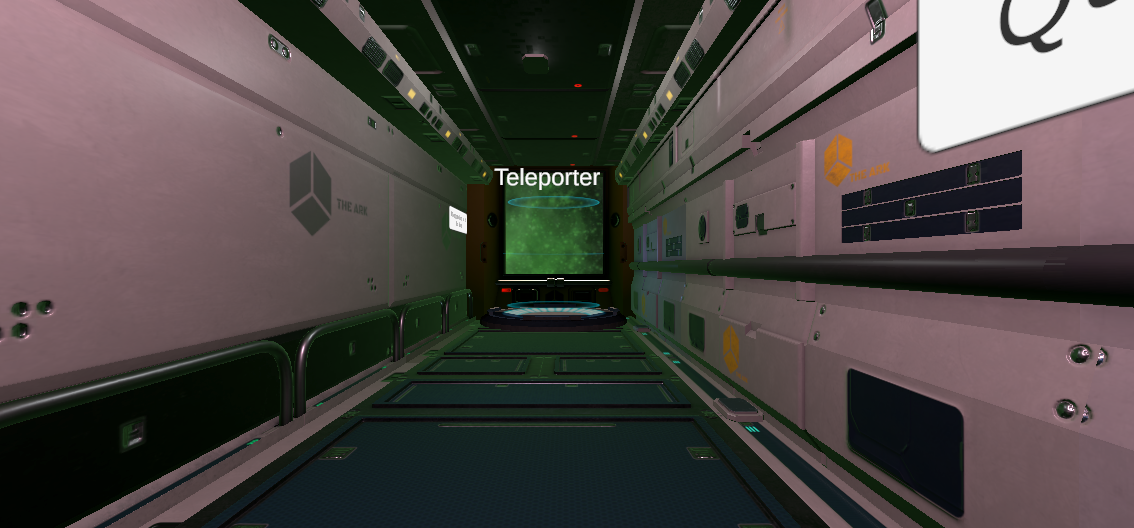
\includegraphics[width= \linewidth]{Figures/HubLoad.png}
  \caption{Main Hub}
  \label{fig:hubload}
\end{figure}

In order to evaluate and test the VR application, there were a series of tests done that allowed us to see the functionality of the application among the different scenes and interactions. These tests focused on bug fixes, motion, and coordination as well as environment
layout in order for the scenes to translate well between one another. The tests were done not only on the Oculus Quest 1 and 2 but also with mouse and keyboard so that debugging can go smoother without the use of a headset at all times. The final stages of user interaction
were done with the Oculus Quests.

The first tests were done with the base scenes in order to check that the environment loaded properly. The main issue that occurred happened with colliders. Users, in this case team members, tested to make sure that there was no clipping between any of the objects present in each scene and the camera that
acted as our character. Along with this, we also tested movement so that a user is not dragging any assets because in some cases the colliders caused objects to be flung into different directions instead of staying in one place or being held in the user's hand. This was fixed by editing the type of colliders
applied to the environment and the user so that there is no clipping and there is free movement without any of the disorienting bugs.

The second round of tests came in the form of texturing. With each scene, specifically the desert scene, there were texture issues due to the type of assets used. The assets used were from the Unity Asset Store and were not optimized for VR. This caused the textures to load in pink indicating that there is an error
with the texture itself. As a result, we tested on different machines first to make sure it was not one user then Melanie proceeded to fix the textures by changing the type of texture applied to the assets. This was done by changing the type of texture from "Standard" to "Unlit" which allowed the textures to load properly. As well as making
sure the textures were not force updated in order to comply with the current version of Unity used for the project.


The final tests were done on two main components that bring the scenes together along with their quests. The first focus was on the main teleportation hub and user interfeace. The main hub was tested to make sure that the teleportation pads were working properly and that the user was able to teleport to each scene. This was done through testing handled by Chethram where
a user stood on a pad to be sent to a scene through a script. However, the teleportation pads were not working properly and the user was not being sent to the correct scene at certain times. This was fixed by changing the script to a button above the pads. This allowed the user to press the button during the rare chance the pads do not work when a user is standing on it.

\begin{figure}[ht!]
  \centering
  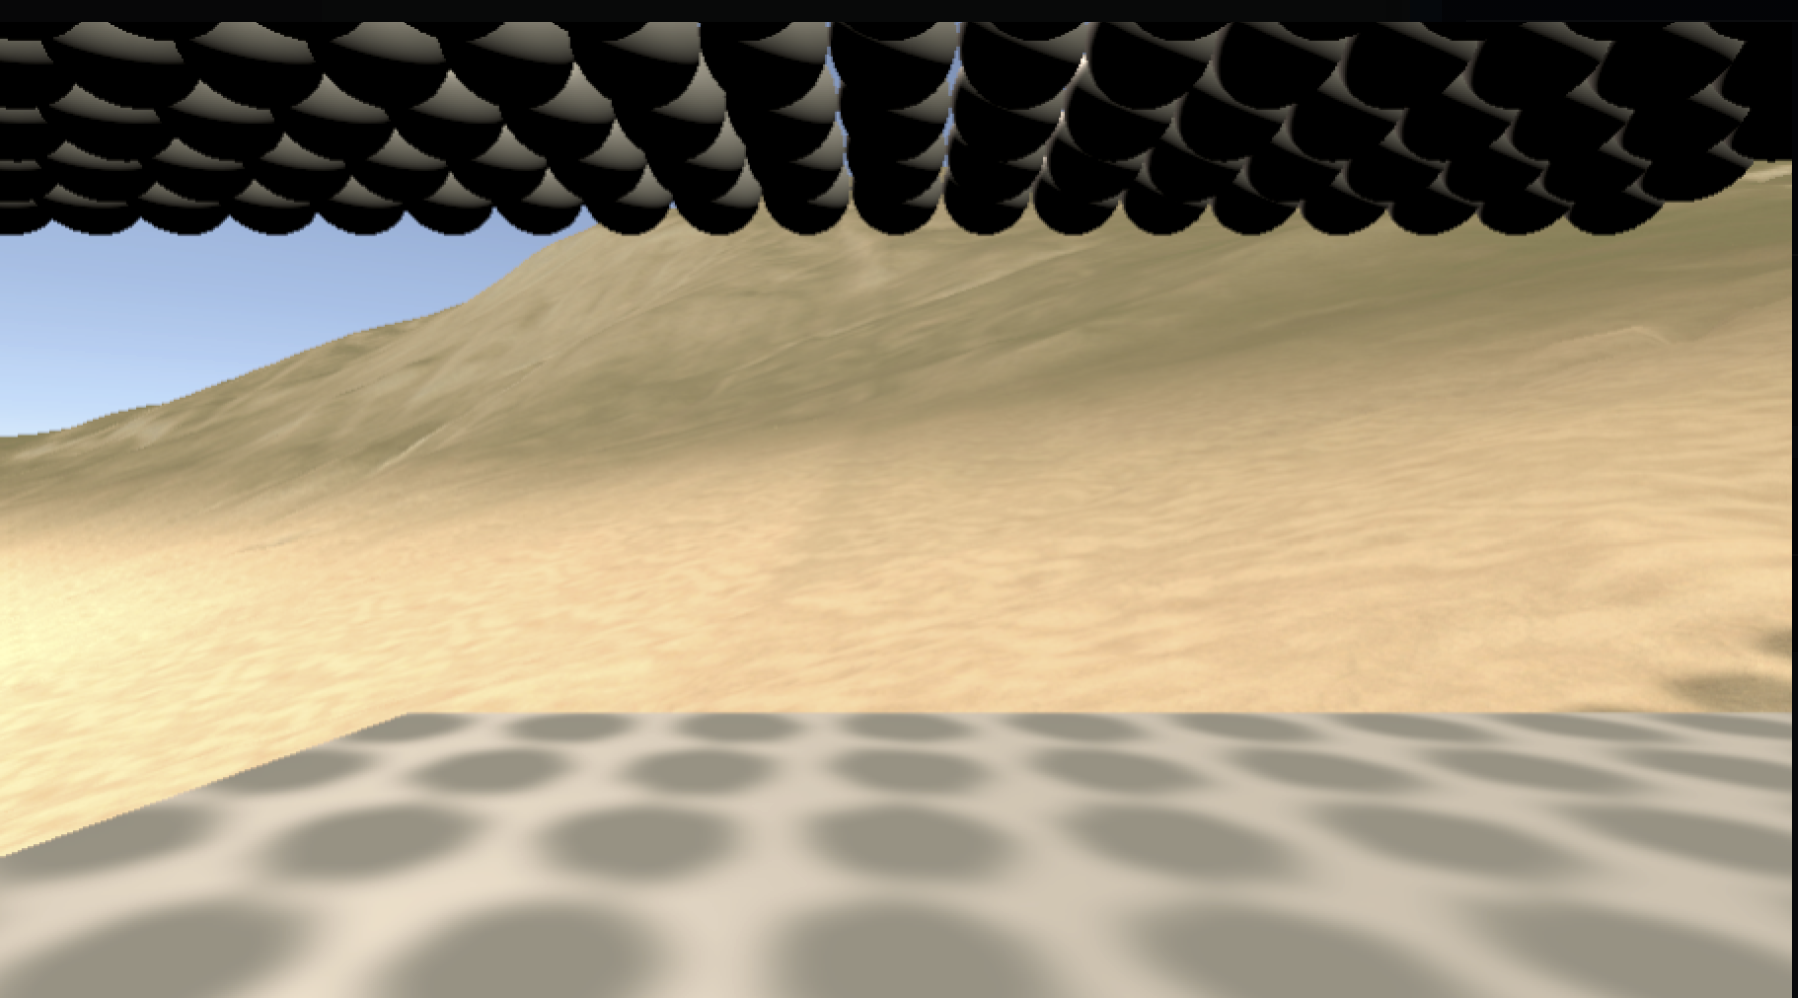
\includegraphics[width= 0.8\linewidth]{Figures/SpawnerBug.png}
  \caption{Spawn Error}
  \label{fig:spawnbug}
\end{figure}

The second focus was on the quests themselves. The quests were tested to make sure that the user was able to collect the items and that the items were being spawned properly. Specifically, we wanted to make sure that the scripts ran for item randomization were efficient enough to make the fetching aspect of the quests interesting for the user. Omar oversaw the creation of the script and tested
different spawn rates as well as items to see how that would affect the spawner in each environment. An issue shown in Fig.\ref{fig:spawnbug} occurred where the spawner would spawn a large number of the items rather than a set number of items within an environment. This could cause large lag spikes when a user spawned in and would often make the game unplayable as time goes on. This was fixed by tweaking
the script in order to not randomize the number of items but rather set the locations manually so that the randomization did not affect the items themselves. This acted as a temporary solution to the problem before fully integrating randomization to the items themselves.

\subsection*{Results}

After taking the time to go through these bugs there was more cohesive gameplay that occured. The items were in the correct locations and the fetching aspects showed no major bugs that affected the overrall experience of the game. Along with that, the ability to have all the environments blend into each other in the form of a space quest logistically supported the use of multiple environments without
throwing off users whenever they tested the game. The script used on the items also showed no problems such as the spawning error and the game was able to only show a select number of items rather than chunks of the same item in incorrect areas. This helped with the exploration aspect as it allowed users to move beyond the spawn point without problem.

\section{Conclusion}
\subsection*{Future Work}
After the completion of the project, there are still a few things that can be done to improve the overall experience of the game. The first is the addition of more NPC interactions outside of the single stranger within the main hub. So far, the NPC interactions have been limited to the stranger in the main hub without others in the different environments. This can make the feeling of the game more desolate than lively
which can be a problem when trying to build immersion within a space. Since the game is not meant to display this sense of loneliness, there can be an inclusion of wildlife that roam around or more individuals that can be communicated with in each environment for future iterations.

Lastly, we aim to expnad on the randomization and possibly integrate it with small side quests that are outside the main fetching quest. This can help build quests that allow for different types of user input that is not solely stuck on head and hand tracking. This can be done through the use of quests focused on things like eye tracking or intense motions like throwing. That way there is more interaction involved within
the game that can be built upong with the ever growing technology related to specific user input. It will also make each environmet more physically interesting rather than visually interesting.

%% if specified like this the section will be committed in review mode
\acknowledgments{
  The authors wish to thank A, B, and C. This work was supported in part by
  a grant from XYZ.}

%\bibliographystyle{abbrv}
\bibliographystyle{ieeetr}
%\bibliographystyle{abbrv-doi-narrow}
%\bibliographystyle{abbrv-doi-hyperref}
%\bibliographystyle{abbrv-doi-hyperref-narrow}

\bibliography{template}
\end{document}
